\section{moeo\-NSGAII$<$ MOEOT $>$ Class Template Reference}
\label{classmoeoNSGAII}\index{moeoNSGAII@{moeoNSGAII}}
The NSGA-II algorithm as described in: Deb, K., S.  


{\tt \#include $<$moeo\-NSGAII.h$>$}

Inheritance diagram for moeo\-NSGAII$<$ MOEOT $>$::\begin{figure}[H]
\begin{center}
\leavevmode
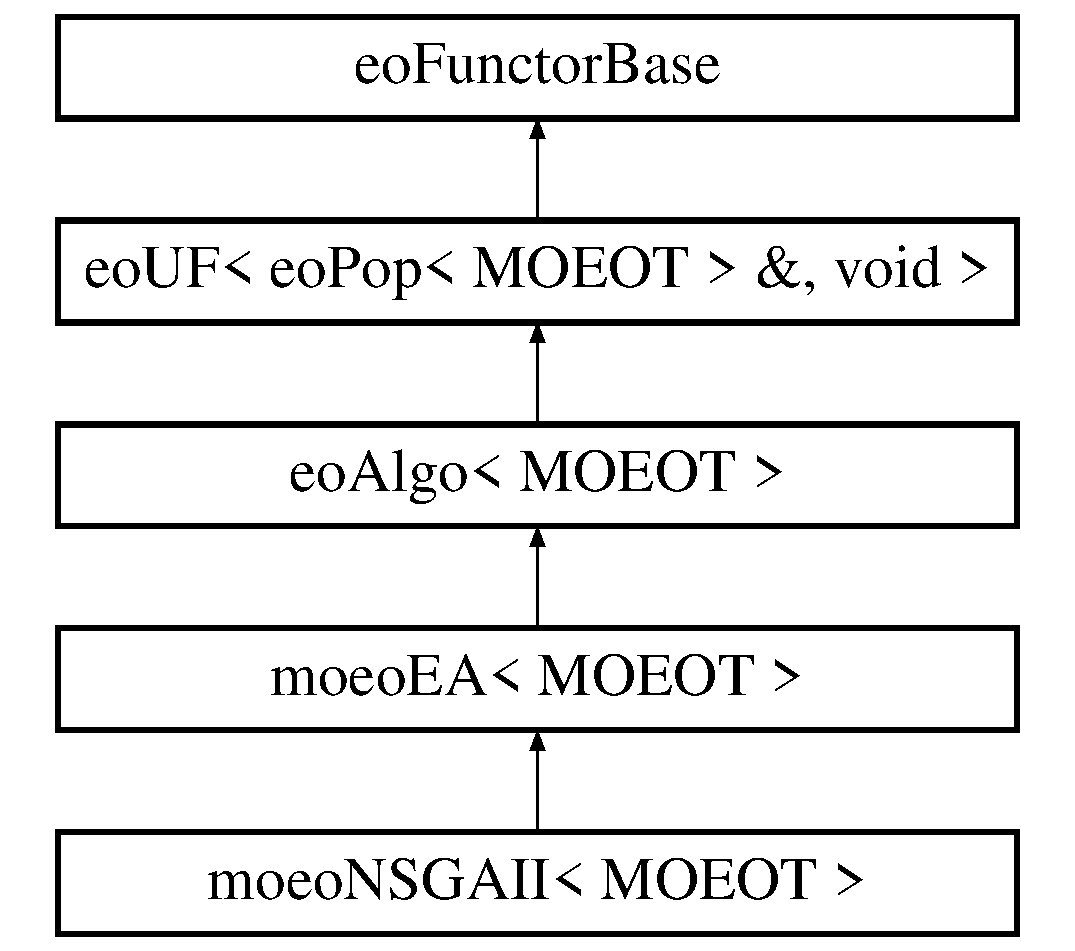
\includegraphics[height=5cm]{classmoeoNSGAII}
\end{center}
\end{figure}
\subsection*{Public Member Functions}
\begin{CompactItemize}
\item 
{\bf moeo\-NSGAII} (unsigned \_\-max\_\-gen, {\bf eo\-Eval\-Func}$<$ MOEOT $>$ \&\_\-eval, {\bf eo\-Gen\-Op}$<$ MOEOT $>$ \&\_\-op)
\begin{CompactList}\small\item\em This constructor builds the algorithm as descibed in the paper. \item\end{CompactList}\item 
{\bf moeo\-NSGAII} (unsigned \_\-max\_\-gen, {\bf eo\-Eval\-Func}$<$ MOEOT $>$ \&\_\-eval, {\bf eo\-Quad\-Op}$<$ MOEOT $>$ \&\_\-crossover, double \_\-p\-Cross, {\bf eo\-Mon\-Op}$<$ MOEOT $>$ \&\_\-mutation, double \_\-p\-Mut)
\begin{CompactList}\small\item\em Ctor taking \_\-max\_\-gen, crossover and mutation. \item\end{CompactList}\item 
{\bf moeo\-NSGAII} ({\bf eo\-Continue}$<$ MOEOT $>$ \&\_\-continuator, {\bf eo\-Eval\-Func}$<$ MOEOT $>$ \&\_\-eval, {\bf eo\-Gen\-Op}$<$ MOEOT $>$ \&\_\-op)
\begin{CompactList}\small\item\em Ctor taking a continuator instead of \_\-gen\_\-max. \item\end{CompactList}\item 
virtual void {\bf operator()} ({\bf eo\-Pop}$<$ MOEOT $>$ \&\_\-pop)
\begin{CompactList}\small\item\em Apply a few generation of evolution to the population \_\-pop. \item\end{CompactList}\end{CompactItemize}
\subsection*{Protected Attributes}
\begin{CompactItemize}
\item 
{\bf eo\-Continue}$<$ MOEOT $>$ \& {\bf continuator}\label{classmoeoNSGAII_7eb1e36631eebbe3216167b1077e3a53}

\begin{CompactList}\small\item\em stopping criteria \item\end{CompactList}\item 
{\bf eo\-Eval\-Func}$<$ MOEOT $>$ \& {\bf eval}\label{classmoeoNSGAII_ae15222c7c9d4a5c3d43df39ad73e008}

\begin{CompactList}\small\item\em evaluation function \item\end{CompactList}\item 
{\bf eo\-Pop\-Loop\-Eval}$<$ MOEOT $>$ {\bf loop\-Eval}\label{classmoeoNSGAII_2e278f1cd90394099b13850ad612104d}

\begin{CompactList}\small\item\em to evaluate the whole population \item\end{CompactList}\item 
{\bf eo\-Pop\-Eval\-Func}$<$ MOEOT $>$ \& {\bf pop\-Eval}\label{classmoeoNSGAII_2926b2c13fbf66aa34ca8bb2d1268df4}

\begin{CompactList}\small\item\em to evaluate the whole population \item\end{CompactList}\item 
{\bf moeo\-Det\-Tournament\-Select}$<$ MOEOT $>$ {\bf select}\label{classmoeoNSGAII_6134c5baa1c6921aaacd67f6f452871a}

\begin{CompactList}\small\item\em binary tournament selection \item\end{CompactList}\item 
{\bf moeo\-Elitist\-Replacement}$<$ MOEOT $>$ {\bf replace}\label{classmoeoNSGAII_75bc4b735c5de2a6fc93b2f2b63c7251}

\begin{CompactList}\small\item\em elitist replacement \item\end{CompactList}\item 
{\bf eo\-General\-Breeder}$<$ MOEOT $>$ {\bf gen\-Breed}\label{classmoeoNSGAII_2099c3069a7da12485578fc66ff71ff1}

\begin{CompactList}\small\item\em general breeder \item\end{CompactList}\item 
{\bf eo\-Breed}$<$ MOEOT $>$ \& {\bf breed}\label{classmoeoNSGAII_17954849435e579d74bf37ed7b9063fc}

\begin{CompactList}\small\item\em breeder \item\end{CompactList}\item 
{\bf moeo\-Fast\-Non\-Dominated\-Sorting\-Fitness\-Assignment}$<$ MOEOT $>$ {\bf fitness\-Assignment}\label{classmoeoNSGAII_2cf7c853cc4213664b0654b1e5a8862a}

\begin{CompactList}\small\item\em fitness assignment used in NSGA-II \item\end{CompactList}\item 
{\bf moeo\-Crowding\-Distance\-Diversity\-Assignment}$<$ MOEOT $>$ {\bf diversity\-Assignment}\label{classmoeoNSGAII_c23794a3b8f5d4845b1153e1fa03dc8c}

\begin{CompactList}\small\item\em Diversity assignment used in NSGA-II. \item\end{CompactList}\end{CompactItemize}


\subsection{Detailed Description}
\subsubsection*{template$<$class MOEOT$>$ class moeo\-NSGAII$<$ MOEOT $>$}

The NSGA-II algorithm as described in: Deb, K., S. 

Agrawal, A. Pratap, and T. Meyarivan : \char`\"{}A fast elitist non-dominated sorting genetic algorithm for multi-objective optimization: NSGA-II\char`\"{}. In IEEE Transactions on Evolutionary Computation, Vol. 6, No 2, pp 182-197 (April 2002). This class builds the NSGA-II algorithm only by using the components of the Paradis\-EO-MOEO framework. 



Definition at line 36 of file moeo\-NSGAII.h.

\subsection{Constructor \& Destructor Documentation}
\index{moeoNSGAII@{moeo\-NSGAII}!moeoNSGAII@{moeoNSGAII}}
\index{moeoNSGAII@{moeoNSGAII}!moeoNSGAII@{moeo\-NSGAII}}
\subsubsection{\setlength{\rightskip}{0pt plus 5cm}template$<$class MOEOT$>$ {\bf moeo\-NSGAII}$<$ MOEOT $>$::{\bf moeo\-NSGAII} (unsigned {\em \_\-max\_\-gen}, {\bf eo\-Eval\-Func}$<$ MOEOT $>$ \& {\em \_\-eval}, {\bf eo\-Gen\-Op}$<$ MOEOT $>$ \& {\em \_\-op})\hspace{0.3cm}{\tt  [inline]}}\label{classmoeoNSGAII_c080a3ce03bfa2a91685e2cf2f0ee75a}


This constructor builds the algorithm as descibed in the paper. 

\begin{Desc}
\item[Parameters:]
\begin{description}
\item[{\em \_\-max\_\-gen}]number of generations before stopping \item[{\em \_\-eval}]evaluation function \item[{\em \_\-op}]variation operator \end{description}
\end{Desc}


Definition at line 46 of file moeo\-NSGAII.h.\index{moeoNSGAII@{moeo\-NSGAII}!moeoNSGAII@{moeoNSGAII}}
\index{moeoNSGAII@{moeoNSGAII}!moeoNSGAII@{moeo\-NSGAII}}
\subsubsection{\setlength{\rightskip}{0pt plus 5cm}template$<$class MOEOT$>$ {\bf moeo\-NSGAII}$<$ MOEOT $>$::{\bf moeo\-NSGAII} (unsigned {\em \_\-max\_\-gen}, {\bf eo\-Eval\-Func}$<$ MOEOT $>$ \& {\em \_\-eval}, {\bf eo\-Quad\-Op}$<$ MOEOT $>$ \& {\em \_\-crossover}, double {\em \_\-p\-Cross}, {\bf eo\-Mon\-Op}$<$ MOEOT $>$ \& {\em \_\-mutation}, double {\em \_\-p\-Mut})\hspace{0.3cm}{\tt  [inline]}}\label{classmoeoNSGAII_3a5800c46a4c66bd2de7111d7cad885b}


Ctor taking \_\-max\_\-gen, crossover and mutation. 

\begin{Desc}
\item[Parameters:]
\begin{description}
\item[{\em \_\-max\_\-gen}]number of generations before stopping \item[{\em \_\-eval}]evaluation function \item[{\em \_\-crossover}]crossover \item[{\em \_\-p\-Cross}]crossover probability \item[{\em \_\-mutation}]mutation \item[{\em \_\-p\-Mut}]mutation probability \end{description}
\end{Desc}


Definition at line 61 of file moeo\-NSGAII.h.\index{moeoNSGAII@{moeo\-NSGAII}!moeoNSGAII@{moeoNSGAII}}
\index{moeoNSGAII@{moeoNSGAII}!moeoNSGAII@{moeo\-NSGAII}}
\subsubsection{\setlength{\rightskip}{0pt plus 5cm}template$<$class MOEOT$>$ {\bf moeo\-NSGAII}$<$ MOEOT $>$::{\bf moeo\-NSGAII} ({\bf eo\-Continue}$<$ MOEOT $>$ \& {\em \_\-continuator}, {\bf eo\-Eval\-Func}$<$ MOEOT $>$ \& {\em \_\-eval}, {\bf eo\-Gen\-Op}$<$ MOEOT $>$ \& {\em \_\-op})\hspace{0.3cm}{\tt  [inline]}}\label{classmoeoNSGAII_1797f01afde01d155e559522df12ae05}


Ctor taking a continuator instead of \_\-gen\_\-max. 

\begin{Desc}
\item[Parameters:]
\begin{description}
\item[{\em \_\-continuator}]stopping criteria \item[{\em \_\-eval}]evaluation function \item[{\em \_\-op}]variation operator \end{description}
\end{Desc}


Definition at line 73 of file moeo\-NSGAII.h.

\subsection{Member Function Documentation}
\index{moeoNSGAII@{moeo\-NSGAII}!operator()@{operator()}}
\index{operator()@{operator()}!moeoNSGAII@{moeo\-NSGAII}}
\subsubsection{\setlength{\rightskip}{0pt plus 5cm}template$<$class MOEOT$>$ virtual void {\bf moeo\-NSGAII}$<$ MOEOT $>$::operator() ({\bf eo\-Pop}$<$ MOEOT $>$ \& {\em \_\-pop})\hspace{0.3cm}{\tt  [inline, virtual]}}\label{classmoeoNSGAII_60ba3ed4287efe81e1ff66b22e1d2e14}


Apply a few generation of evolution to the population \_\-pop. 

\begin{Desc}
\item[Parameters:]
\begin{description}
\item[{\em \_\-pop}]the population \end{description}
\end{Desc}


Implements {\bf eo\-UF$<$ eo\-Pop$<$ MOEOT $>$ \&, void $>$}.

Definition at line 83 of file moeo\-NSGAII.h.

References moeo\-NSGAII$<$ MOEOT $>$::breed, moeo\-NSGAII$<$ MOEOT $>$::continuator, moeo\-NSGAII$<$ MOEOT $>$::diversity\-Assignment, moeo\-NSGAII$<$ MOEOT $>$::fitness\-Assignment, moeo\-NSGAII$<$ MOEOT $>$::pop\-Eval, and moeo\-NSGAII$<$ MOEOT $>$::replace.

The documentation for this class was generated from the following file:\begin{CompactItemize}
\item 
moeo\-NSGAII.h\end{CompactItemize}
